\documentclass[]{article}
\usepackage{fullpage}
\usepackage[authoryear]{natbib}
\usepackage{setspace}
    \doublespacing
\usepackage{hyperref}
\hypersetup{
    colorlinks,
    citecolor=black,
    filecolor=black,
    linkcolor=cyan,
    urlcolor=cyan
}
\usepackage{amssymb,amsmath}
\usepackage{bm}
\usepackage{dcolumn}
\usepackage{booktabs}
\usepackage{url}
\usepackage{tikz}
\usepackage{todonotes}
\usepackage[utf8]{inputenc}
\usepackage{graphicx}
\usepackage{longtable}
\usepackage{todonotes}
\usepackage{lscape}
\usepackage{float}


\title{Tell Them When You're Safe: Elections and revealing the costs of financial crises}
\author{Christopher Gandrud and Mark Hallerberg \\ \emph{Hertie School of Governance}\footnote{Please contact Christopher Gandrud
(\href{mailto:gandrud@hertie-school.org}{\nolinkurl{gandrud@hertie-school.org}}).
Our research is generously supported by the Deutsche Forschungsgemeinschaft.
All data and replication material can be found at:
\url{https://github.com/christophergandrud/EIUCrisesMeasure}.}}

\begin{document}

\maketitle


\textbf{Incomplete Working Draft}

\begin{abstract}
How do elections and electoral competitiveness affect governments' fiscal decisions during financial crises? Some previous research has found that having competitive elections reduces the costs of financial crises. The idea is that politicians need to keep costs low to please taxpaying voters. However, governments have plenty of avenues to obscure costs and so have some degree of control over when costs are revealed. We reexamine the relationship between elections and fiscal responses to financial crises in OECD countries using a novel approach to measuring changes in government liabilities as a result of financial stress. We find that governments do change their budgetary behaviour in response to elections in that they are more likely to expose more liabilities when they are as safe as possible. Public liabilities from responding to financial market stress noticeably increase immediately following elections.

\end{abstract}

[INTRODUCTION]

\section{Previous research on elections and financial crisis fiscal policy}

[POLITICAL BUDGET CYCLES]

[FISCAL RESPONSES TO CRISES]

[SOMETHING LIKE 1.3 and 1.4 FROM THE WEP PAPER]

\begin{quote}
        $H_{1}$: Immediately following elections, governments will have larger fiscal liabilities in response to to financial market stress.
\end{quote}

\section{Measurement}

It is difficult to accurately measure the occurrence and intensity of financial crises, as well as fiscal response to these crises. In this section we describe these difficulties as well as our innovative approach to overcoming them. We then discuss the right-hand variables we use to help explain these choices.

\subsection*{Measuring Fiscal Responses to Financial Crises}



Perhaps the most prominent research on the political economy of responding to financial crisis is \cite{Keefer2007}. He aimed to understand how competitive elections possibly lowered these costs. Given that the costs of responding to financial crises are significant--likely approaching 40 percent of GDP in some countries during the recent crisis \cite{laeven2013}--it is surprising that few other pieces of research have tried to understand how politics and political institutions shape crisis costs.

Perhaps a contributing factor to the dearth of research trying to understand the fiscal costs of financial crises is that it is very difficult to actually pin down what these costs are. Perhaps the main source of fiscal crisis costs comes from an ongoing, though irregular IMF/World Bank data set on financial crises. The most recent version is \cite{laeven2013}, which includes a fiscal costs variable as a percentage of GDP. An earlier version of this data set was used in \cite{Keefer2007}. A difficulty for researchers using this data is that it that it cost estimates for a particular crisis can change dramatically over time. \cite{GandrudHallerberg2015} demonstrate that significant revisions have been made to this data set, such that when updated data is used Keefer's \citeyearpar{Keefer2007} results regarding competitive elections having a negative affect on costs disappear.

It is so difficult to accurately pin down the costs of crises partially because responding to financial crisis often does not involve direct spending, e.g. the government giving taxpayer money directly to troubled banks to strengthen their balance sheets, but issuing new liabilities by for example lending money to banks that it borrowed. The ultimate costs of these liabilities are affected by a complex and interactive set of factors, only some of which a particular government can control. Ultimate costs can be affected by the initial size and type of the liabilities, the severity of the crisis, the competency of government bureaucracies that administer them, internal and external economic developments including global liquidity shocks, and successor government decisions to change policies, such as closing a public bad bank earlier than planned possibly resulting in the assets being sold at lower prices. It is very difficult to accurately attribute costs to a particular government that develop over many years and are affected by many factors outside of the government's control.

Governments can use policies that create contingent liabilities--e.g. guarantees--that have some probability of being converted to actual liabilities. This probability is partially affected by government competence, but also exogenous factors such as global credit conditions. Contingent liabilities can also often be obscured from government debt statistics, so it is almost impossible to conduct cross-country research on what factors affect these probabilities. \cite{gandrudHallerbergWEP} argue that the use of contingent liabilities can be endogenous to political environments, with governments facing elections more likely to use them. They additionally so that definitions of what constitute contingent and realised liabilities furthermore varies across time and place depending on public finance accounting regimes.

We take a new approach to measuring fiscal responses to financial crises. Rather than focusing on final costs, which are difficult to ascribe to choices of particular governments and which may be the result of disparate accounting regimes, we focus on deviations from average government liabilities and spending per year, given economic conditions. This approach is based on the underlying assumption that all governments--particularly in advanced democracies who need to please voters with an interest in economic stability \cite{Rosas2009}--respond to economic shocks by increasing their spending and liabilities. This can be from a combination of automatic shock responses, such as unemployment insurance and deposit insurance, as well as new allocations to, for example, purchase toxic assets from trouble banks or provide them with liquidity assistance. We should expect that there will be a larger fiscal response the more sever the crisis. Given that we should expect all governments in advanced democracies to respond to economic shocks and more to larger shocks, we are interested in examining how political factors affect government decisions to do more (or less) than the average response at a given level of crisis severity.

Before discussing the specific way we measure deviations from trend fiscal policies, it is important to note that both our interest in policy responses in advanced democracies and data availability combine to constrict our sample to 30 OECD member countries from 2003 through 2011. Please see the Online Appendix for the full list. These countries had a wide range of experiences with financial crises over this time period.

We estimate trend fiscal responses to financial market stress by first gathering data on general government liabilities--debt and other liabilities--and spending per country-year from the OECD.\footnote{Data was accessed through \url{https://data.oecd.org/} in June 2015.} Separate data on ``economic affairs'' spending is available, so we focus on that as it the most relevant spending quantity. The original variables were expressed as percentages of GDP. To isolate changes to fiscal policy, rather than GDP, we transformed the variables to be in terms of each country's 2005 GDP.\footnote{GDP data was from the OECD. Accessed June 2015.}

\begin{table}
    \caption{Linear Regressions to Create Government Liability and Spending Residuals}
    \label{liab_resid}

    \begin{center}
        
% Table created by stargazer v.5.1 by Marek Hlavac, Harvard University. E-mail: hlavac at fas.harvard.edu
% Date and time: Thu, Jun 18, 2015 - 15:19:06
\begingroup 
\footnotesize 
\begin{tabular}{@{\extracolsep{5pt}}lcccc} 
\\[-1.8ex]\hline 
\hline \\[-1.8ex] 
 & \multicolumn{4}{c}{\textit{Dependent variable:}} \\ 
\cline{2-5} 
\\[-1.8ex] & $\Delta$ Liabilities & $\Delta$ Liabilities Resid. & $\Delta$ Econ. Spend & $\Delta$ Econ. Spend Resid. \\ 
\\[-1.8ex] & (1) & (2) & (3) & (4)\\ 
\hline \\[-1.8ex] 
 Output Gap & $-$0.430$^{***}$ &  & 0.209$^{***}$ &  \\ 
  & (0.105) &  & (0.054) &  \\ 
  & & & & \\ 
 Perceived Financial Stress &  & 10.383$^{***}$ &  & 0.656 \\ 
  &  & (2.992) &  & (1.644) \\ 
  & & & & \\ 
 Constant & 2.937 & $-$5.582$^{**}$ & 0.708 & $-$0.353 \\ 
  & (1.897) & (2.446) & (0.984) & (1.322) \\ 
  & & & & \\ 
\hline \\[-1.8ex] 
country fixed effects & Yes & Yes & Yes & Yes \\ 
\hline \\[-1.8ex] 
Observations & 240 & 240 & 223 & 223 \\ 
R$^{2}$ & 0.274 & 0.055 & 0.114 & 0.001 \\ 
Adjusted R$^{2}$ & 0.170 & $-$0.081 & $-$0.025 & $-$0.155 \\ 
Residual Std. Error & 5.362 (df = 209) & 5.213 (df = 209) & 2.782 (df = 192) & 2.780 (df = 192) \\ 
F Statistic & 2.632$^{***}$ (df = 30; 209) & 0.402 (df = 30; 209) & 0.820 (df = 30; 192) & 0.005 (df = 30; 192) \\ 
\hline 
\hline \\[-1.8ex] 
\textit{Note:}  & \multicolumn{4}{r}{$^{*}$p$<$0.1; $^{**}$p$<$0.05; $^{***}$p$<$0.01} \\ 
\end{tabular} 
\endgroup 

    \end{center}

\end{table}

Financial crises and economic growth shocks are highly related \cite[see][]{Reinhart2009}. We separated out the trend responses to economic growth shocks by first regressing the output gap\footnote{Output gap data was from the OECD. Accessed June 2015.} on liabilities and spending using a partial adjustment model that also included the lagged dependent variable. The first and second columns of Figure~\ref{liab_resid} show coefficient estimates from these regressions. We can see that a worsening output gap is associated with increases in government liabilities. Worsening output gaps are are associated with spending increases, though not statistically significantly.

We then took residuals from these two models and used them in similar partial adjustment regression models with a measure of perceived financial market stress. The measure is from \cite{gandrudHallEPFMS}. They conduct a textual analysis of monthly Economist Intelligence Unit (EIU) country reports to develop an index of real-time perceptions of financial market stress that they call the EIU Perceptions of Financial Market Stress (EPFMS) from 2003 through 2011. The EPFMS Index ranges from zero--low stress--to 1--high stress. We found the annual mean of the monthly observations of the EPFMS Index to make it comparable to the annual OECD budget data. Please see \cite{gandrudHallEPFMS} for a review of other measures of financial market stress and crisis and a justification for why their measure is preferable for studying policy responses. We can see in the third column of Table~\ref{liab_resid} that perceived financial market stress is very strongly positively associated with the residuals from the output gap-liabilities regression,\footnote{The residuals range from about -16 to 45, with the inter-quartile range of about 5.} i.e. increases in financial market stress have an important effect on increases in government liabilities that are not explained by drops in economic output. As expected, these results indicate that governments are taking on liabilities to support financial markets in addition to the broader economy. Perceived financial market stress is also associated with the residual of changes in spending.

We focus on residuals from models three and four in Table~\ref{liab_resid} as our dependent variables of interest. These residuals can be thought of as deviations from average liabilities and spending at given levels of output gaps and financial market stress. We further transform the variable by finding the year-on-year change in these variables as we are most interested in how governments change their fiscal policies.

\subsection*{Right-hand variables}

Our primary right-hand variables of interest are government election year and post-election year dummies. This data is based on the election timing variable from \cite{gandrudYrcurnt}. We anticipate that governments will decrease (increase) their realised fiscal policy in election (post-election) years.

The mechanism behind this possible relationship is how safe politicians feel they are from being removed from office. To further examine this possible mechanism, we also include the probability that the plurality party will be removed from its plurality position in the next election from the perspective of immediately after the previous election. This data is from \cite{Kayser2015comp}. We furthermore interacted this variable with the election/post-election variables.\footnote{The relevant interactions are election year and lagged loss probability and post-election year and current loss probability.} Governments that are facing an imminent election and have a high loss probability are very insecure. Conversely, those who have just survived an election and have a low loss probability are very secure.

We include a number of other variables in an attempt to control for omitted variable bias. \cite{broz2013} finds some evidence that government ideology can affect policy responses to financial crises, in particular that economically left-wing governments increase regulation. Perhaps governments of different ideological stripes respond to financial market stress with different fiscal policy changes. The affect of partisanship is possibly ambiguous, however. The traditional left-right divide on fiscal policy may breakdown in regards to financial crises, both may have an interest in economic stability, possibly inclining them to support banks. Regardless, this is an empirical issue that we examine by including the Database of Political Institution's \citep[][updated through 2012]{DPI2001} government economic ideology variable. It is one for right-wing governments, two for centrist governments, and three for those on the left.

Governments may be constrained in their ability to actually change fiscal policy in a given year in response to economic shocks \cite[e.g.][]{MacIntyre2001}. If there are more checks on a government then they might not be able to change fiscal policy as they otherwise would like to. So, we include a measure of political constraints from \cite[][updated through 2011]{Henisz2004}.\footnote{We specifically used the POLCONIII variable.}

[...]

\section{Regression results}

\begin{figure}
    \caption{Marginal Effect of Elections on Non-Trend Fiscal Responses to Perceived Financial Market Stress}
    \label{me_liab_stress}

    \begin{center}
        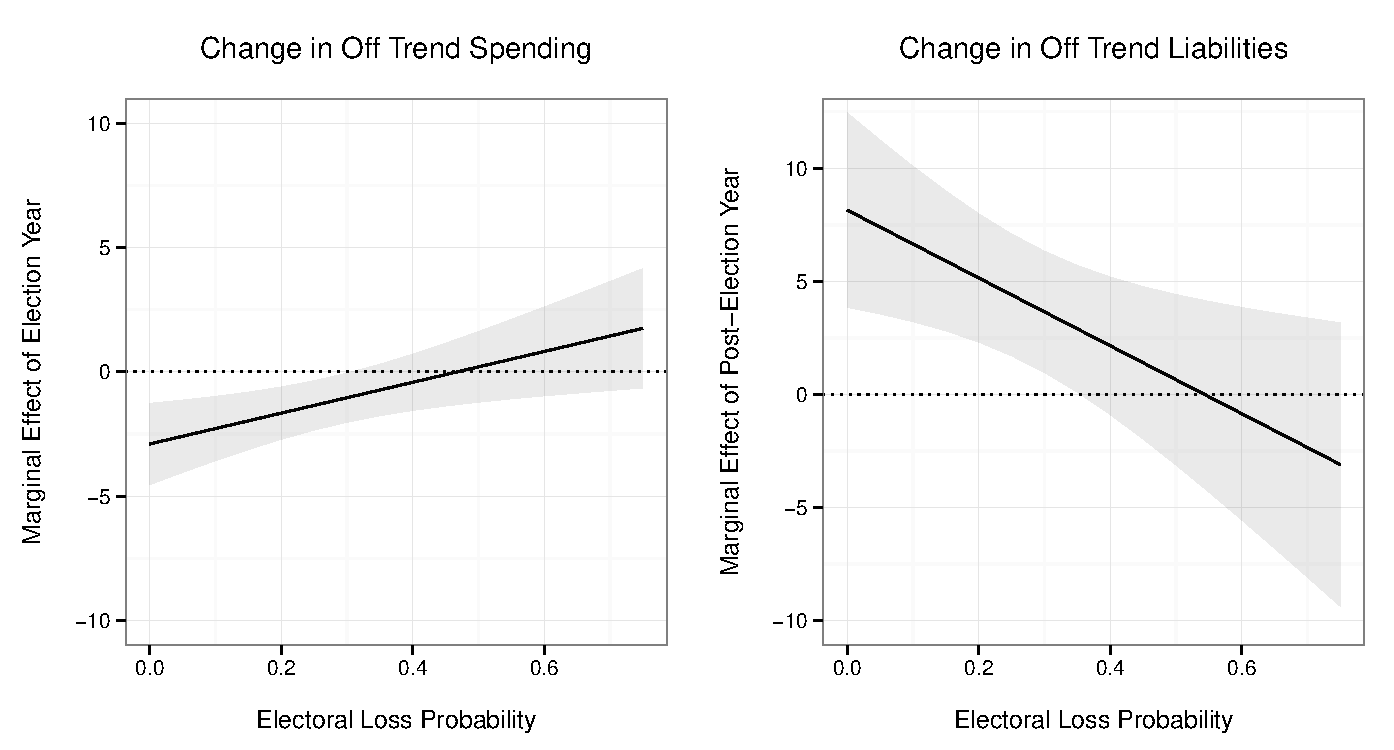
\includegraphics[scale=0.7]{analysis/figures/me_stress.pdf}
    \end{center}

    {\scriptsize{Shadded areas represent 90\% confidence intervals. \\
    Plots made using model 2 in Table~\ref{t1_stress}.}}

\end{figure}

\begin{table}
    \caption{Linear Regression of Non-Trend Fiscal Responses to Perceived Financial Market Stress (election year)}
    \label{t0_stress}

    \begin{center}
        
% Table created by stargazer v.5.1 by Marek Hlavac, Harvard University. E-mail: hlavac at fas.harvard.edu
% Date and time: Thu, Jun 18, 2015 - 17:04:34
\begingroup 
\footnotesize 
\begin{tabular}{@{\extracolsep{5pt}}lccc} 
\\[-1.8ex]\hline 
\hline \\[-1.8ex] 
 & \multicolumn{3}{c}{\textit{Dependent variable:}} \\ 
\cline{2-4} 
\\[-1.8ex] & (1) & (2) & (3)\\ 
\hline \\[-1.8ex] 
 Election Yr. & $-$1.819$^{*}$ & $-$4.389$^{**}$ & $-$4.415$^{**}$ \\ 
  & (1.062) & (1.921) & (1.954) \\ 
  & & & \\ 
 Loss Prob. (lag 1) & $-$4.070 & $-$6.366$^{*}$ & $-$6.829$^{*}$ \\ 
  & (3.481) & (3.752) & (3.897) \\ 
  & & & \\ 
 Econ Ideology &  &  & $-$0.031 \\ 
  &  &  & (0.484) \\ 
  & & & \\ 
 Political Constraints &  &  & $-$2.828 \\ 
  &  &  & (4.766) \\ 
  & & & \\ 
 Election Yr. * Loss Prob. &  & 7.895 & 8.033 \\ 
  &  & (4.925) & (5.012) \\ 
  & & & \\ 
 Constant & 1.840 & 2.551 & 4.143 \\ 
  & (2.191) & (2.227) & (3.831) \\ 
  & & & \\ 
\hline \\[-1.8ex] 
country fixed effects & Yes & Yes & Yes \\ 
\hline \\[-1.8ex] 
Observations & 240 & 240 & 232 \\ 
R$^{2}$ & 0.021 & 0.033 & 0.035 \\ 
Adjusted R$^{2}$ & $-$0.125 & $-$0.117 & $-$0.126 \\ 
Residual Std. Error & 5.171 (df = 208) & 5.152 (df = 207) & 5.238 (df = 198) \\ 
F Statistic & 0.142 (df = 31; 208) & 0.219 (df = 32; 207) & 0.217 (df = 33; 198) \\ 
\hline 
\hline \\[-1.8ex] 
\textit{Note:}  & \multicolumn{3}{r}{$^{*}$p$<$0.1; $^{**}$p$<$0.05; $^{***}$p$<$0.01} \\ 
\end{tabular} 
\endgroup 

    \end{center}

\end{table}

\begin{table}
    \caption{Linear Regression of Non-Trend Fiscal Responses to Perceived Financial Market Stress (post-election year)}
    \label{t1_stress}

    \begin{center}
        
% Table created by stargazer v.5.1 by Marek Hlavac, Harvard University. E-mail: hlavac at fas.harvard.edu
% Date and time: Thu, Jun 18, 2015 - 17:04:35
\begingroup 
\footnotesize 
\begin{tabular}{@{\extracolsep{5pt}}lccc} 
\\[-1.8ex]\hline 
\hline \\[-1.8ex] 
 & \multicolumn{3}{c}{\textit{Dependent variable:}} \\ 
\cline{2-4} 
\\[-1.8ex] & (1) & (2) & (3)\\ 
\hline \\[-1.8ex] 
 Post-Election Yr. & 2.150$^{**}$ & 6.514$^{***}$ & 6.507$^{***}$ \\ 
  & (1.022) & (1.866) & (1.898) \\ 
  & & & \\ 
 Loss Prob. & $-$4.634 & $-$0.639 & $-$0.777 \\ 
  & (3.547) & (3.776) & (3.853) \\ 
  & & & \\ 
 Econ Ideology &  &  & 0.017 \\ 
  &  &  & (0.476) \\ 
  & & & \\ 
 Political Constraints &  &  & $-$1.916 \\ 
  &  &  & (4.668) \\ 
  & & & \\ 
 Election Yr. * Loss Prob. &  & $-$13.196$^{***}$ & $-$13.321$^{***}$ \\ 
  &  & (4.755) & (4.852) \\ 
  & & & \\ 
 Constant & 1.118 & 0.016 & 0.972 \\ 
  & (2.227) & (2.228) & (3.668) \\ 
  & & & \\ 
\hline \\[-1.8ex] 
country fixed effects & Yes & Yes & Yes \\ 
\hline \\[-1.8ex] 
Observations & 240 & 240 & 232 \\ 
R$^{2}$ & 0.028 & 0.062 & 0.064 \\ 
Adjusted R$^{2}$ & $-$0.117 & $-$0.083 & $-$0.092 \\ 
Residual Std. Error & 5.154 (df = 208) & 5.072 (df = 207) & 5.158 (df = 198) \\ 
F Statistic & 0.190 (df = 31; 208) & 0.431 (df = 32; 207) & 0.410 (df = 33; 198) \\ 
\hline 
\hline \\[-1.8ex] 
\textit{Note:}  & \multicolumn{3}{r}{$^{*}$p$<$0.1; $^{**}$p$<$0.05; $^{***}$p$<$0.01} \\ 
\end{tabular} 
\endgroup 

    \end{center}

\end{table}


\section*{Conclusion}




%%%%%%%%%%%% Bibliography %%%%%%%%%%%%%%
\bibliographystyle{apsr}
\bibliography{main.bib}

\section{Online Appendix}

% latex table generated in R 3.2.0 by xtable 1.7-4 package
% Thu Jun 18 17:04:35 2015
\begin{table}[ht]
\centering
\caption{Regressions Country Sample} 
\label{country_sample}
{\footnotesize
\begin{tabular}{l}
  \hline
Country \\ 
  \hline
Australia \\ 
  Austria \\ 
  Belgium \\ 
  Canada \\ 
  Czech Republic \\ 
  Denmark \\ 
  Estonia \\ 
  Finland \\ 
  France \\ 
  Germany \\ 
  Greece \\ 
  Hungary \\ 
  Iceland \\ 
  Ireland \\ 
  Israel \\ 
  Italy \\ 
  Japan \\ 
  Korea, Republic of \\ 
  Luxembourg \\ 
  Netherlands \\ 
  New Zealand \\ 
  Norway \\ 
  Poland \\ 
  Portugal \\ 
  Slovakia \\ 
  Slovenia \\ 
  Spain \\ 
  Sweden \\ 
  Switzerland \\ 
  United Kingdom \\ 
   \hline
\end{tabular}
}
\end{table}


\end{document}
